\documentclass[xcolor=dvipsnames]{article}
\usepackage{tikz,pgf}
\usetikzlibrary{snakes,shapes,trees,shadows,arrows,positioning,decorations.pathreplacing,automata}
\colorlet{shadecolor}{gray!20}
\usepackage[paperwidth=7.5in, paperheight=4.75in, top=0.1in, bottom=0.1in, left=0.1in, right=0.1in]{geometry}

\begin{document}
\thispagestyle{empty}
\tikzstyle{every picture}+=[remember picture]


\tikzstyle{na} = [baseline=-.5ex]
\tikzstyle{civ}=[circle, fill=gray!10, minimum size=2.5cm]
\tikzstyle{com}=[circle, fill=gray!20, minimum size=2.5cm]
\tikzstyle{init} = [pin edge={to-,thin,white}]


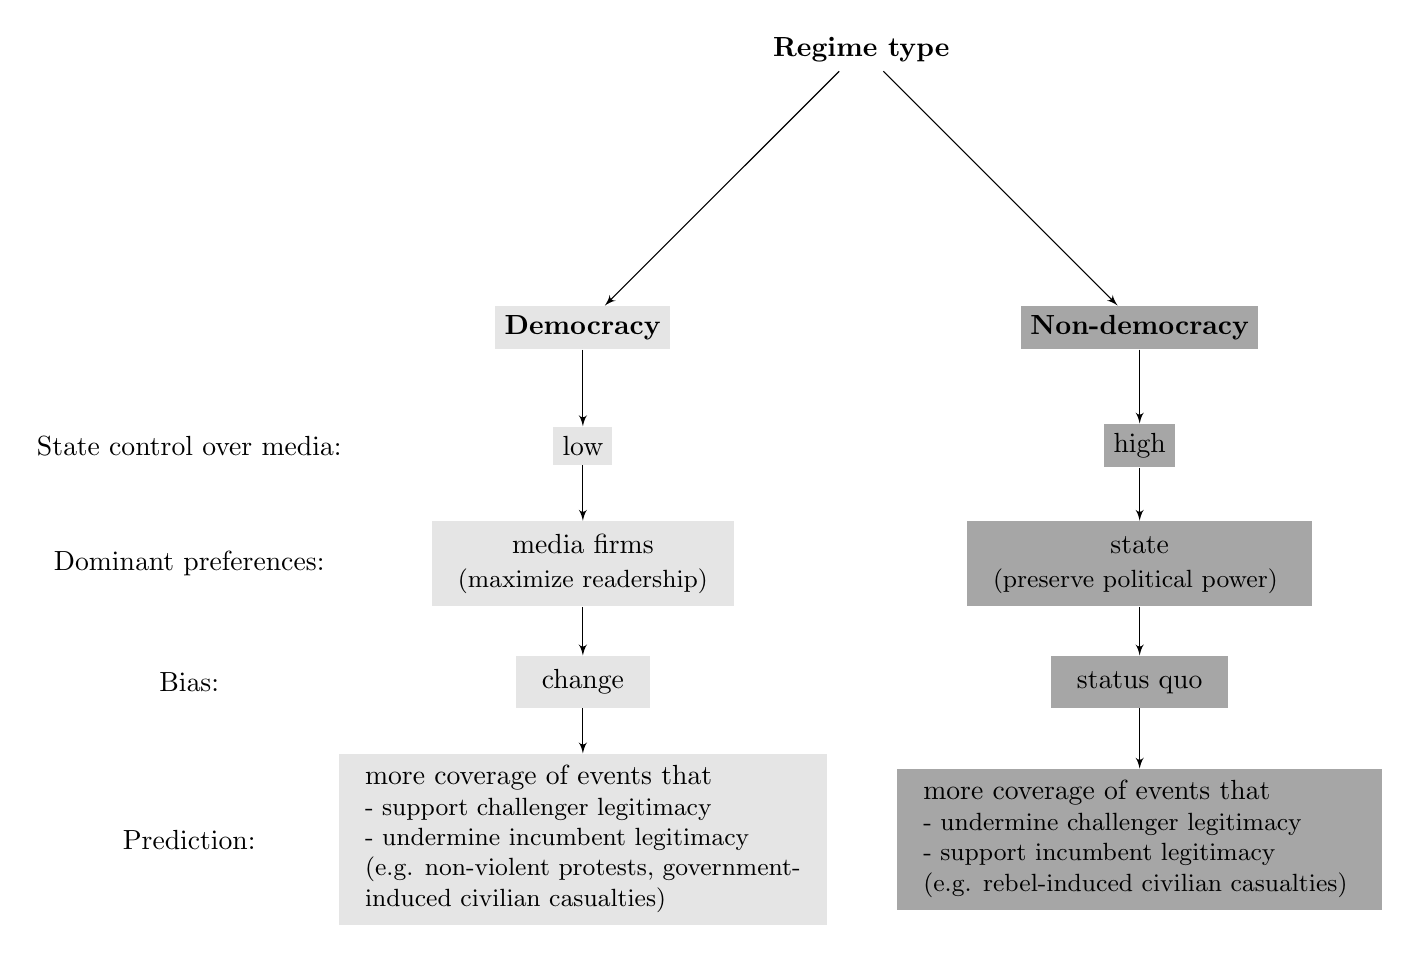
\begin{tikzpicture}[node distance=3.2cm,auto,>=latex']
    \node [fill=white] (r) {\textbf{Regime type}};
    %%%%%%%%%
    \node (d) [fill=gray!20, below left of=r, node distance=5cm]{\textbf{Democracy}};
        \node (d1) [fill=gray!20, below of=d, node distance=1.5cm]{low};
        \node (d2) [fill=gray!20, below of=d1, node distance=1.5cm]{\begin{tabular}{c}
     media firms \\
     \small{(maximize readership)} \\
  \end{tabular}};
        \node (d3) [fill=gray!20, below of=d2, node distance=1.5cm]{\begin{tabular}{c}
     change \\
  \end{tabular}};
        \node (d4) [fill=gray!20, below of=d3, node distance=2cm]{\small\begin{tabular}{l}
     \normalsize{more coverage of events that}\\
     - support challenger legitimacy \\    
         - undermine incumbent legitimacy \\
     (e.g. non-violent protests, government-\\
          induced civilian casualties) \\
  \end{tabular}};  %%%%%%%%%
    \node (nd) [fill=gray!70, below right of=r, node distance=5cm]{\textbf{\textcolor{black}{Non-democracy}}};
        \node (nd1) [fill=gray!70, below of=nd, node distance=1.5cm]{\textcolor{black}{high}}; 
        \node (nd2) [fill=gray!70, below of=nd1, node distance=1.5cm]{\begin{tabular}{c}
    \textcolor{black}{state} \\
     \textcolor{black}{\small{(preserve political power)} }\\
  \end{tabular}};
        \node (nd3) [fill=gray!70, below of=nd2, node distance=1.5cm]{\begin{tabular}{c}
     \textcolor{black}{status quo} \\
  \end{tabular}};
        \node (nd4) [fill=gray!70, below of=nd3, node distance=2cm]{\small\begin{tabular}{l}
     \textcolor{black}{\normalsize{more coverage of events that}}\\
     \textcolor{black}{- undermine challenger legitimacy} \\    
        \textcolor{black}{ - support incumbent legitimacy }\\
    \textcolor{black}{ (e.g. rebel-induced civilian casualties) }\\
  \end{tabular}};
  %%%%%%%%%%
        \node (a0) [left of=d1, node distance=5cm]{State control over media:};
        \node (b0) [below of=a0, node distance=1.5cm]{Dominant preferences:};        
        \node (c0) [below of=b0, node distance=1.5cm]{Bias:};        
        \node (d0) [below of=c0, node distance=2cm]{Prediction:};       
            \draw[->] (r) edge  (d);
            \draw[->] (d) edge  (d1);
            \draw[->] (d1) edge  (d2);
            \draw[->] (d2) edge  (d3);
            \draw[->] (d3) edge  (d4);
            \draw[->] (r) edge  (nd);        
            \draw[->] (nd) edge  (nd1);
            \draw[->] (nd1) edge  (nd2);
            \draw[->] (nd2) edge  (nd3);
            \draw[->] (nd3) edge  (nd4);
\end{tikzpicture}

\end{document}